% ドキュメントの設定
\documentclass[a4paper,11pt,xelatex,ja=standard]{bxjsarticle}
\usepackage{tikz}
\usetikzlibrary {datavisualization.formats.functions}
\usepackage{pgfplots}
\usepackage{float}
\usepackage{amsmath}

% ドキュメント開始
\begin{document}

\section{目的}
    \begin{enumerate}
        \item グラフィカルユーザインタフェース・プログラムによる計測プログラムの作成
        \item サンプリング定理の確認
    \end{enumerate}

\section{方法}

    \begin{enumerate}
        \item データ1・データ2の計測
        \begin{itemize}
            \item 振幅2.0[V]のSIN波をファンクションジェネレータからアナログ0ch(AI0)に入力。
            \item 異なるサンプリング条件で信号を1秒間計測。
            \item 入力信号とサンプリング周波数は表1に従う。
            \item データは「データ1」「データ2」と呼ぶ。
            \item 計測開始前に信号振幅と周波数をオシロスコープで確認。
        \end{itemize}
        \item 合成信号の作成と計測
        \begin{itemize}
            \item ブレッドボード上で二台のファンクションジェネレータの信号を合成。
            \item 信号の設定は表2に従う。
            \item それぞれの信号振幅と周波数はオシロスコープでモニターし、実験中は合成信号を観測。
            \item 合成信号をch0に入力し、異なるサンプリング周波数で計測。
            \item サンプリング周波数の条件は表3に従い、計測時間は1秒。
            \item データは「データ3」「データ4」と呼ぶ。
        \end{itemize}
    \end{enumerate}
    
\section{結果}

    \subsection{150HzのSin波の計測}

        150Hzの正弦波を2kHzのサンプリング周波数でサンプリングした。得られた波形を見ると、150Hzの信号が正しく維持されていることがわかる。
        \begin{figure}[H]
            \centering
            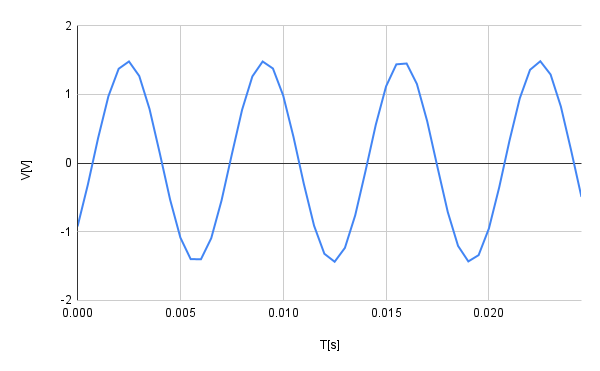
\includegraphics[width=1.0\textwidth]{./img/24-4-2/150HzのSin波を2kHzでサンプリング.png}
            \caption{150HzのSin波を120Hzでサンプリングした結果}
        \end{figure}

        一方、150Hzの正弦波を120Hzのサンプリング周波数でサンプリングした場合、エイリアシング効果により、元の信号が正しく再現されないことがわかります。

        \begin{figure}[H]
            \centering
            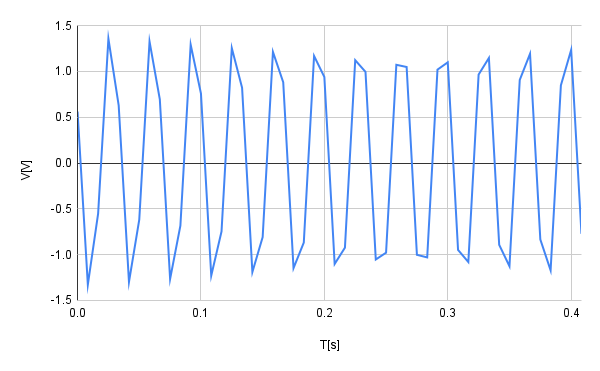
\includegraphics[width=1.0\textwidth]{./img/24-4-2/150HzのSin波を120Hzでサンプリング.png}
            \caption{150HzのSin波を120Hzでサンプリング結果}
        \end{figure}

    \subsection{100Hzと2kHzの合成Sin波}

        100Hzと2kHzの合成正弦波を20kHzのサンプリング周波数でサンプリングしました。得られた波形を見ると、両方の信号が正しく維持されていることが確認できます。


        \begin{figure}[H]
            \centering
            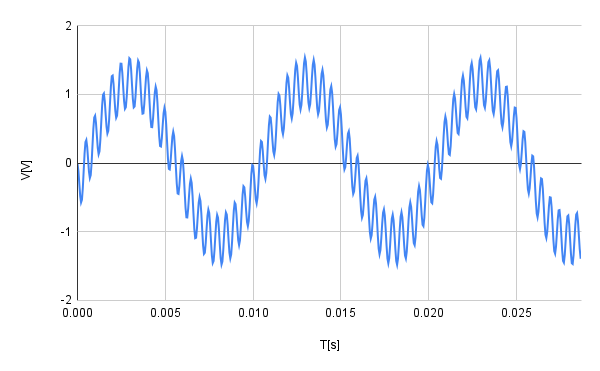
\includegraphics[width=1.0\textwidth]{./img/24-4-2/100Hzと2kHzの合成Sin波を20kHzでサンプリング.png}
            \caption{100Hzと2kHzの合成Sin波を20kHzでサンプリング結果}
        \end{figure}

        一方、100Hzと2kHzの合成正弦波を1800Hzのサンプリング周波数でサンプリングした場合、エイリアシング効果により、元の信号が正しく再現されないことがわかります。

        \begin{figure}[H]
            \centering
            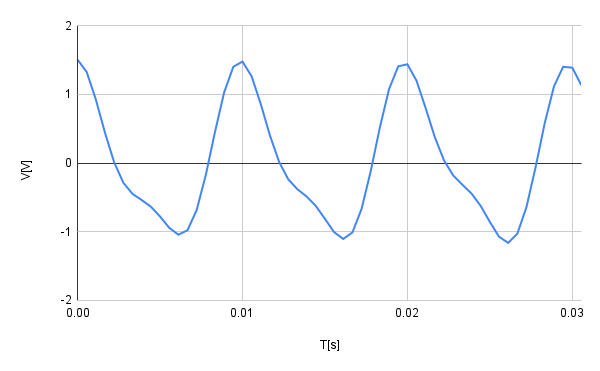
\includegraphics[width=1.0\textwidth]{./img/24-4-2/100Hzと2kHzの合成Sin波を1800Hzでサンプリング.png}
            \caption{100Hzと2kHzの合成Sin波を1800Hzでサンプリング結果}
        \end{figure}

\section{考察}

    \subsection{サンプリングとスペクトルの折り返し現象}

        今回の実験において、150Hzの正弦波を2kHzのサンプリング周波数でサンプリングした結果、元の波形が正しく維持されていることが確認できました。しかし、120Hzのサンプリング周波数でサンプリングした場合、元の信号がエイリアシング効果により正しく再現されないことが観測されました。エイリアシングは、サンプリング定理に反してサンプリング周波数が信号の最大周波数の2倍以上でない場合に発生します。サンプリング周波数が信号周波数よりも低い場合、スペクトルが折り返し現象を起こし、異なる周波数成分として現れるため、元の波形が再現されません。

    \subsection{DFTの結果とスペクトルの関係}

        DFT(離散フーリエ変換)を用いて得られたスペクトルからも、この現象を確認することができます。2kHzのサンプリング周波数で取得したデータに対してDFTを適用すると、150Hzの成分が正しく現れます。しかし、120Hzのサンプリング周波数で取得したデータに対してDFTを適用すると、150Hzの成分が折り返しによって他の周波数成分として現れます。これは、サンプリングによって生じるスペクトルの繰り返しによる影響です。

    \subsection{正しいサンプリング条件の選定}

        100Hzと2kHzの合成信号についても同様の現象が観測されました。20kHzのサンプリング周波数では両方の信号成分が正しく維持されますが、1800Hzのサンプリング周波数ではエイリアシングにより信号が正しく再現されません。このように、サンプリング定理を満たすためには、信号の最大周波数の2倍以上のサンプリング周波数を選定する必要があります。

    \subsection{改善策}

        信号を正しく計測するためには、次のような改善策が考えられます:

        \begin{itemize}
        \item サンプリング周波数を信号の最大周波数の2倍以上に設定する。
        \item エイリアシング防止のためのアンチエイリアシングフィルタを使用し、高周波成分を除去する。
        \end{itemize}

    これにより、サンプリングによる信号の歪みを最小限に抑え、正確な波形情報を得ることができます。

\section{結論}

    \begin{itemize}
        \item サンプリング周波数が信号の最大周波数の2倍以上である場合、信号を正確に再現できることが確認できました。具体的には、150Hzの正弦波を2kHzのサンプリング周波数でサンプリングした結果、元の波形が正しく維持されました。
        \item サンプリング周波数が信号の最大周波数の2倍未満である場合、エイリアシング効果により信号が正しく再現されないことが確認できました。150Hzの正弦波を120Hzでサンプリングした場合、元の信号が歪んでしまいました。
        \item 100Hzと2kHzの合成信号についても同様に、サンプリング周波数が十分に高い場合は信号が正しく維持されますが、低い場合はエイリアシングが発生しました。
        \item エイリアシング効果を防ぐためには、信号の最大周波数の2倍以上のサンプリング周波数を選定することが重要であり、加えてアンチエイリアシングフィルタの使用も有効であることがわかりました。
    \end{itemize}

\end{document}